\documentclass{article}
\usepackage{graphicx}
\usepackage{listings}
\usepackage{color}
\usepackage{amsmath}
\usepackage{amsfonts}
\usepackage{bm}
\usepackage[utf8]{inputenc}

\title{Modelli dinamici Pt.1\\
	Corso di LSMC, a.a. 2017-2018}
\author{Davide Gori\\
	550282}


\definecolor{backcolour}{rgb}{0.95,0.95,0.92}
\definecolor{gray}{rgb}{0.5,0.5,0.5}
\lstset{basicstyle=\ttfamily\small,
	columns=fullflexible,
	numbers=left,
	numberstyle=\tiny\ttfamily\color{gray},
	backgroundcolor=\color{backcolour},
	tabsize=4,
	language=Octave
}


\begin{document}
	\maketitle
	\section{Prima sperimentazione: moto di un paracadutista}
	Si vuole simulare il moto di un paracadutista che viene lanciato da un aereo in volo.
	\begin{itemize}
		\item Altitudine aereo: $1200$ metri.
		\item Istante apertura paracadute: $x_p$.
		\item Coefficiente resistenza aria per $x<x_p$: $k_1=16.4$.
		\item Coefficiente resistenza aria per $x>x_p$: $k_2=180$.
		\item Peso paracadutista: $m=90$ chili.
		
	\end{itemize}
	Studierò il moto del paracadutista supponendo che il paracadute venga aperto nell’istante $xp = 15$.\\
	Risolvendo numericamente il problema sull'intervallo $\left[0, x_max\right]$ mediante il metodo di Runge-Kutta classico e rappresentando graficamente lo spostamento e la velocità sulla stessa figura in due grafici diversi.\\
	Infine stabiliremo il valore di $x_max$ e la velocità del paracadutista al momento dell'atterraggio.\\
	\subsection{L'implementazione}
	L'equazione differenzile è la seguente ({\tt fun}):
	\begin{equation}
	\begin{cases}
	y''= -g-h_1 y' , & t \leq x_p\\
	y''= -g-h_2 y' , & t > x_p\\
	\end{cases}
	\end{equation}
	Dove $h_1=\frac{k_1}{m}=\frac{16.5}{90}$, $h_2=\frac{k_2}{m}=\frac{180}{90}$, $g=9.8$ e $x_p=15$.
	\subsection{Il codice}
	Questo è lo script che realizza lasperimentazione:
	\lstinputlisting{LabSper_5_1.m}
	Dove {\tt fun} è la seguente:
	\lstinputlisting{fun.m}
	\subsection{Risultati}
	Riportiamo il grafico in output.\\
	\begin{figure}[htp!]
		\centering 
		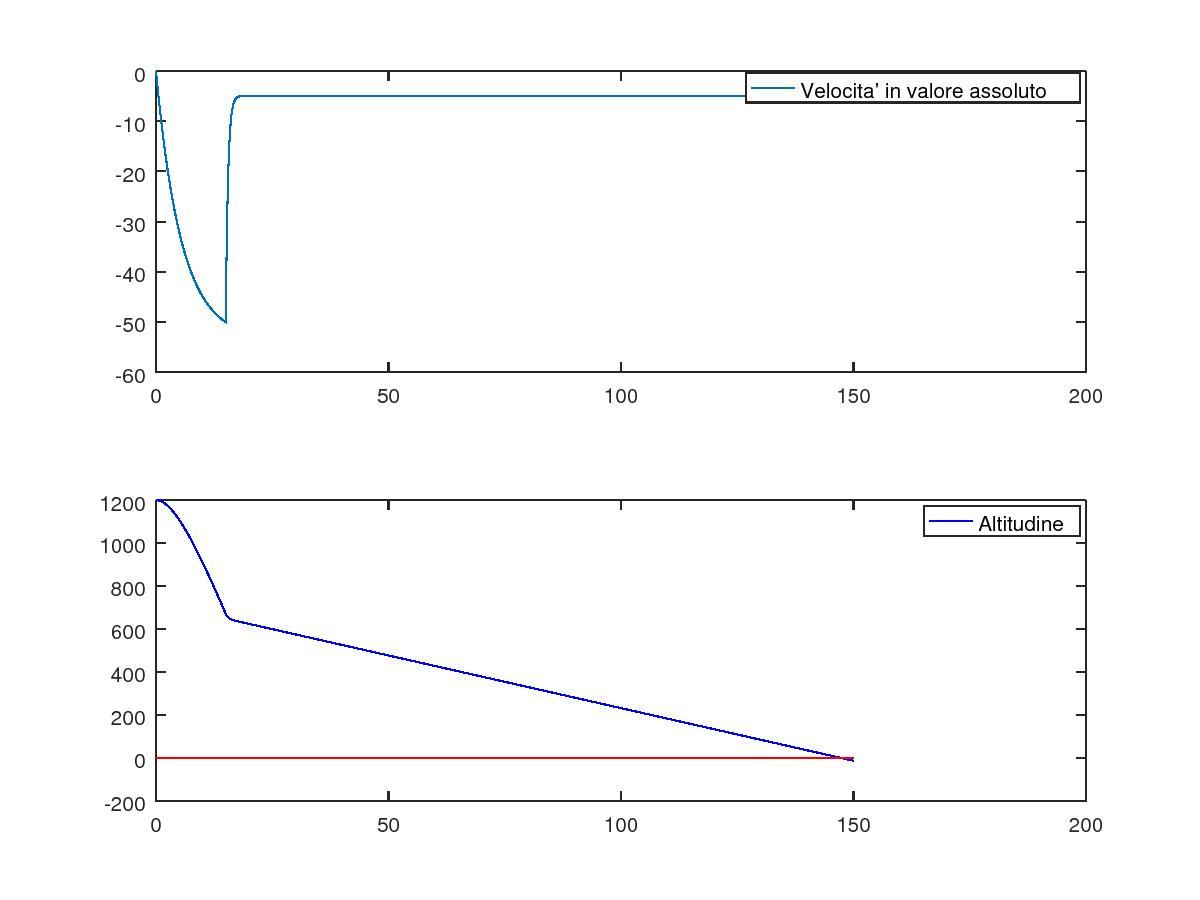
\includegraphics[width=\textwidth]{5_1.jpeg}
	\end{figure}
	\newpage
	Aiutandoci con il grafico e con un po' di tentativi a mano si scopre che:\\
	\begin{itemize}
		\item l'atterraggio avviene al tempo $147.38$.
		\item la velocità all'atterraggio è $y'(147.38)=-4.9$
	\end{itemize}

	\section{Seconda sperimentazione: pendolo semplice}
	Utilizzando la routine ode45, risolverò l’equazione del pendolo semplice associata alle	condizioni iniziali: $y(0)=\frac{\pi}{6}$ e $y'(0)=0$ nell’intervallo $\left[0, 10\right]$, con $l=2$.\\
	Creerò poi un grafico della situazione.\\
	\subsection{L'implementazione}
	L'equazione differenzile è la seguente:
	\begin{equation}
	\begin{cases}
	y''=-k \sin(y) \\
	y(0)=\frac{\pi}{6}\\
	y'(0)=0
	\end{cases}
	\end{equation}
	Dove $k=\frac{g}{l}=\frac{9.8}{2}$.
	
	\subsection{Il codice}
	Questo è lo script che realizza la sperimentazione:
	\lstinputlisting{LabSper_5_2.m}
	
	\subsection{Risultati}
	Riportiamo il grafico in output.\\
	\begin{figure}[htp!]
		\centering 
		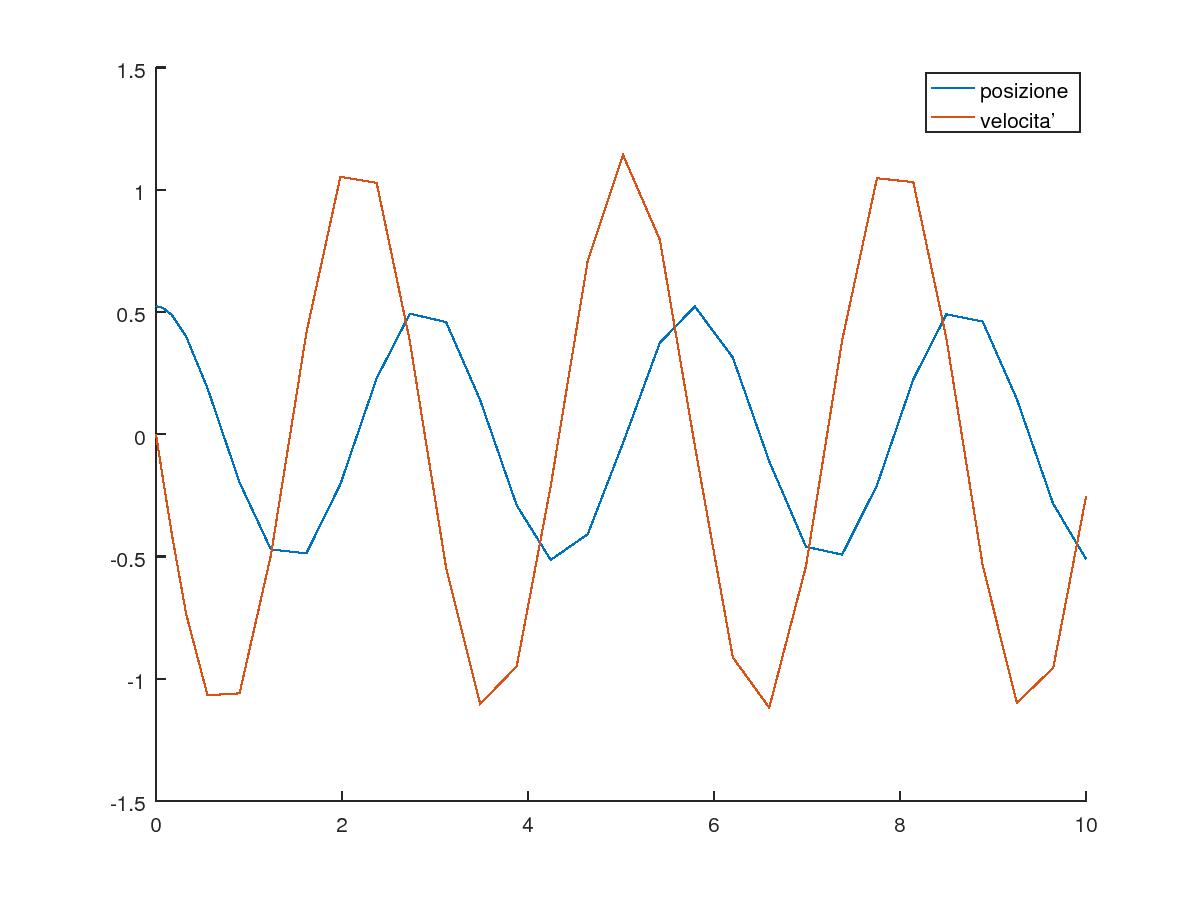
\includegraphics[width=0.5\textwidth]{5_2.jpeg}
	\end{figure}
	
	\section{Terza sperimentazione: pendolo approssimato}
	Ripetiamo la sperimentazione precedente approssimando $\sin(y)$ con $y$. e confrontiamo i due modelli.
	\subsection{L'implementazione}
	L'equazione differenzile è la seguente:
	\begin{equation}
	\begin{cases}
	y''=-k y \\
	y(0)=\frac{\pi}{6}\\
	y'(0)=0
	\end{cases}
	\end{equation}
	Dove $k=\frac{g}{l}=\frac{9.8}{2}$.
	
	\subsection{Il codice}
	Questo è lo script che realizza la sperimentazione:
	\lstinputlisting{LabSper_5_3.m}
	
	\subsection{Risultati}
	Riportiamo il grafico in output.\\
	\begin{figure}[htp!]
		\centering 
		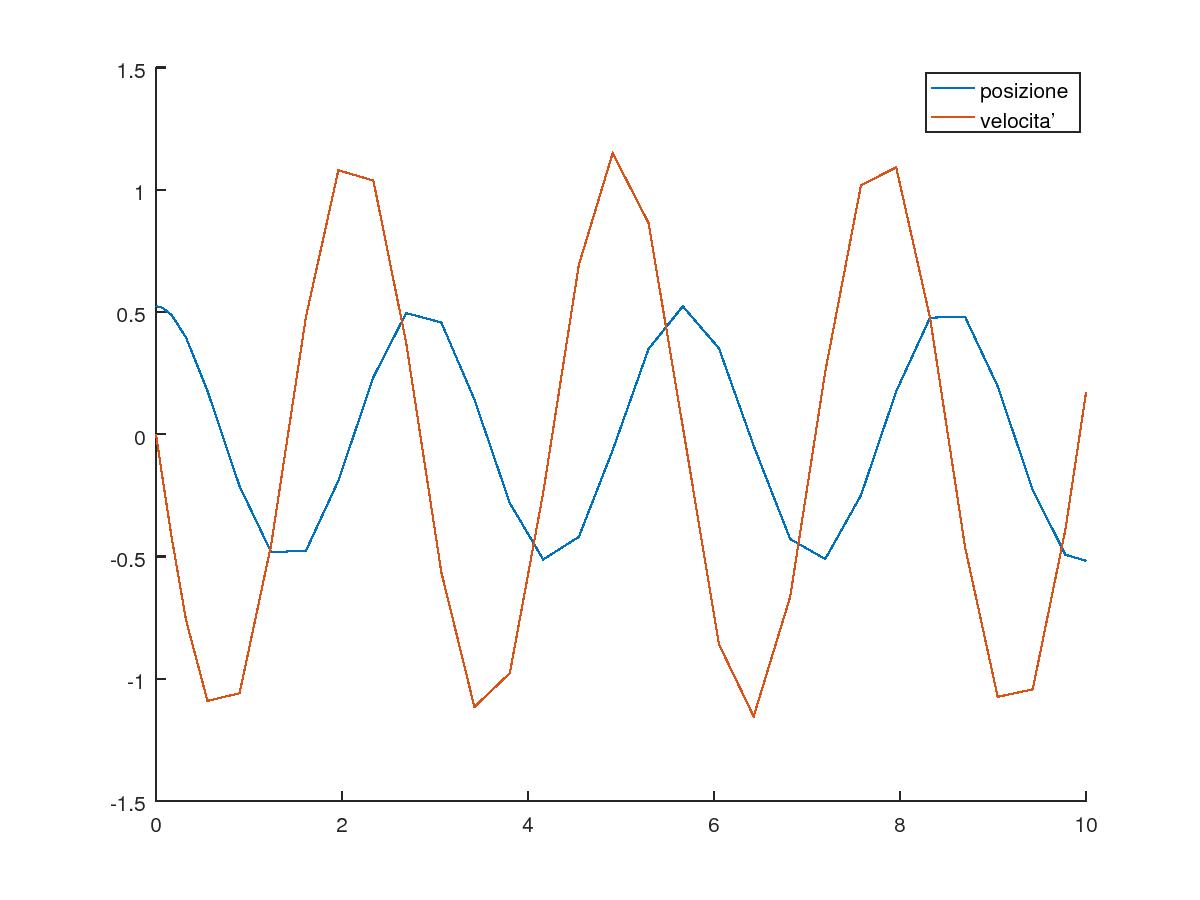
\includegraphics[width=0.5\textwidth]{5_3.jpeg}
	\end{figure}
	Si osserva che la soluzione è molto simile a quella esatta, quindi abbiamo usato una buona approssimazione, cioè $y$ resta piccolo. Si nota comunque che nel caso non approssimato si ha un periodo di oscillazione leggermente più breve.
	
	\section{Quarta sperimentazione: oscillatore armoinco smorzato}
	 considererò l'equazione dell'oscillatore armonico semplice con i parametri fissati come segue:
	 \begin{itemize}
	 	\item oscillatore libero non smorzato: $m=1$, $h=10$, $k=0$, $f = 0$; con condizioni iniziali $y(0) = 1$, $y'(0)=0$ e si osservi il fenomeno nell'intervallo $\left[0, 60\right]$;
	 	\item oscillatore libero sottosmorzato: $m=1$, $h=10$, $k=0.5$, $f = 0$; con condizioni iniziali $y(0) = 1$, $y'(0)=0$ e si osservi il fenomeno nell'intervallo $\left[0, 60\right]$;
	 	\item oscillatore libero sovrasmorzato: $m=1$, $h=10$, $k=10$, $f = 0$; con condizioni iniziali $y(0) = 1$, $y'(0)=0$ e si osservi il fenomeno nell'intervallo $\left[0, 60\right]$;
	 	\item oscillatore libero smorzato: $m=1$, $h=10$, $k=0.75$, $f = 25$; con condizioni iniziali $y(0) = 2$, $y'(0)=0$ e si osservi il fenomeno nell'intervallo $\left[0, 60\right]$;
	 \end{itemize}
	Scriverò un file di tipo script che, per mezzo di un menu, permetta all’utente di scegliere il caso test, i cui parametri
	sono definiti in un ciclo switch. Determinando la soluzione numerica mediante la routine {\tt ode45}. Creerò poi dei grafici delle soluzioni.
	\subsection{Implementazione}
	il modello è il seguente:
	\begin{equation}
	\begin{cases}
	y''=-\frac{k}{m}y'-\frac{g}{h}sin(y)+f \\
	y(0)=y_0 \\
	y'(0)=y'_0 \\
	\end{cases}
	\end{equation}
	\subsection{Il codice}
	Questo è lo script che realizza la sperimentazione:
	\lstinputlisting{LabSper_5_4.m}
	
	\subsection{Risultati}
	Riportiamo i grafici in output.\\
	\begin{figure}[htp!]
		\centering 
		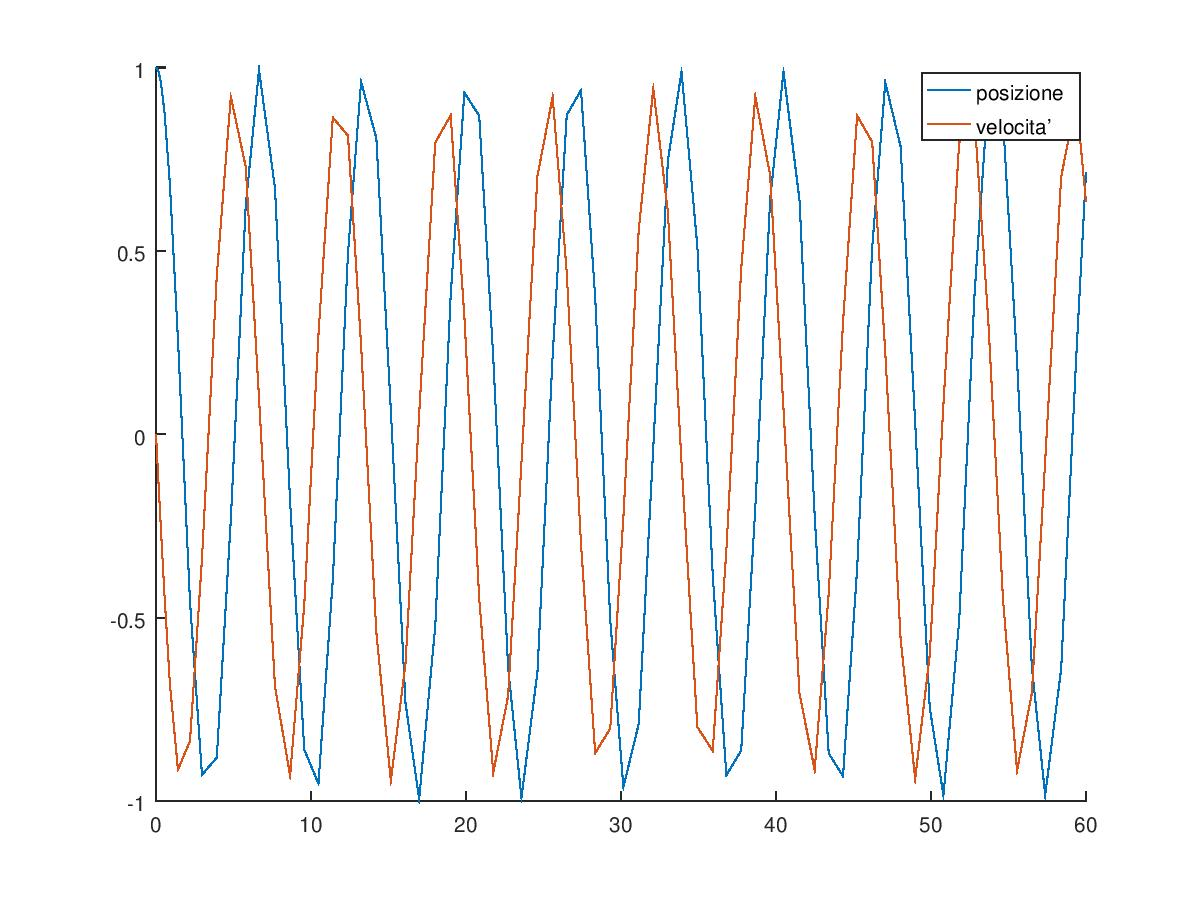
\includegraphics[width=0.7\textwidth]{5_4_1.jpeg}
	\end{figure}
		\begin{figure}[htp!]
		\centering 
		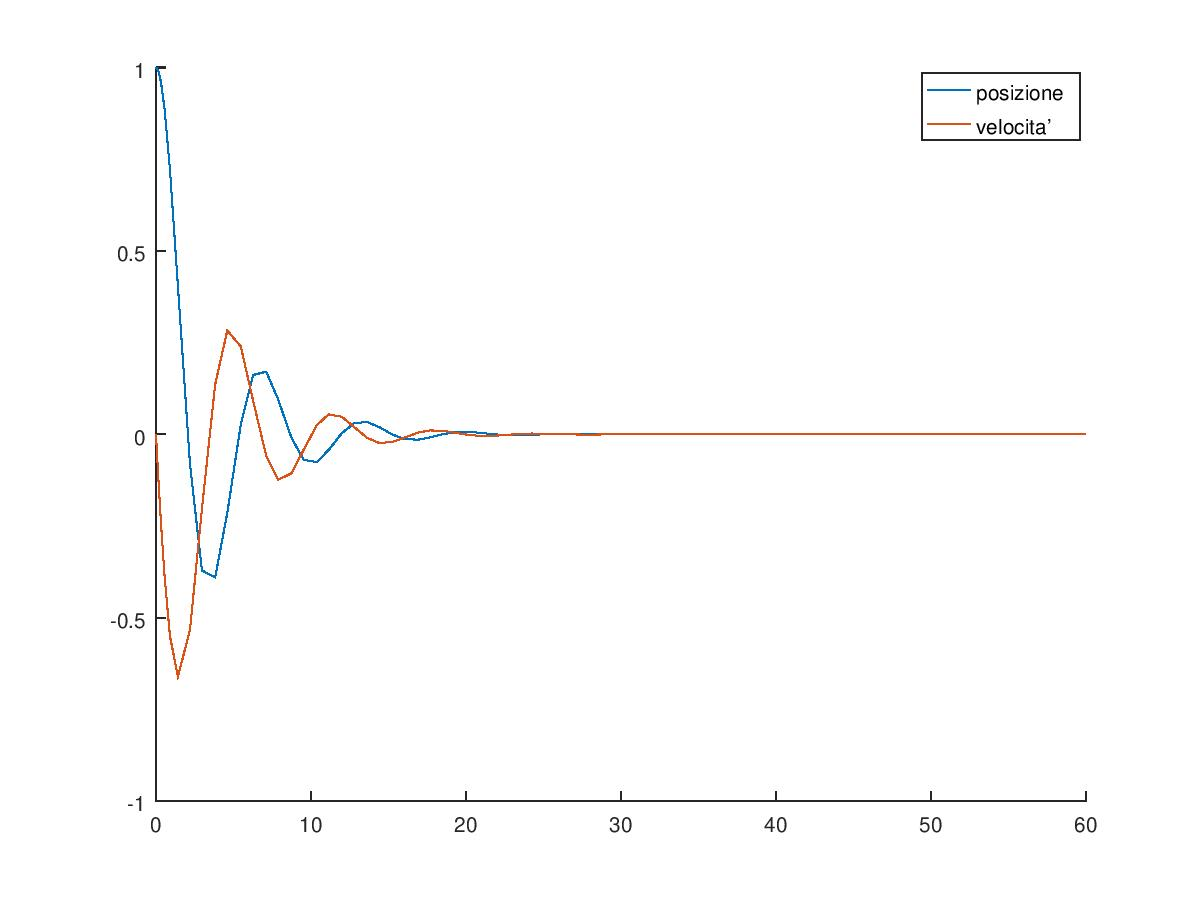
\includegraphics[width=0.7\textwidth]{5_4_2.jpeg}
	\end{figure}
	\begin{figure}[htp!]
		\centering 
		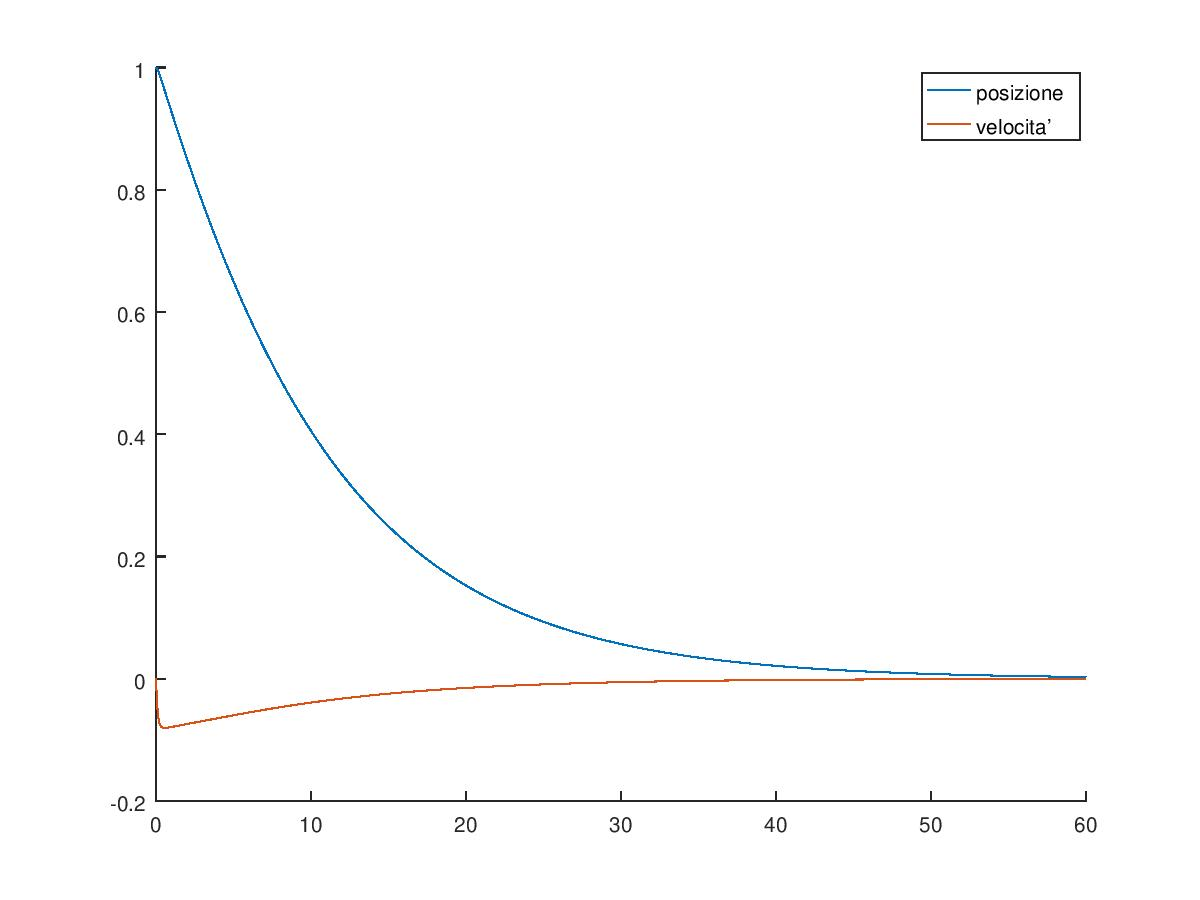
\includegraphics[width=0.7\textwidth]{5_4_3.jpeg}
	\end{figure}
	\begin{figure}[htp!]
		\centering 
		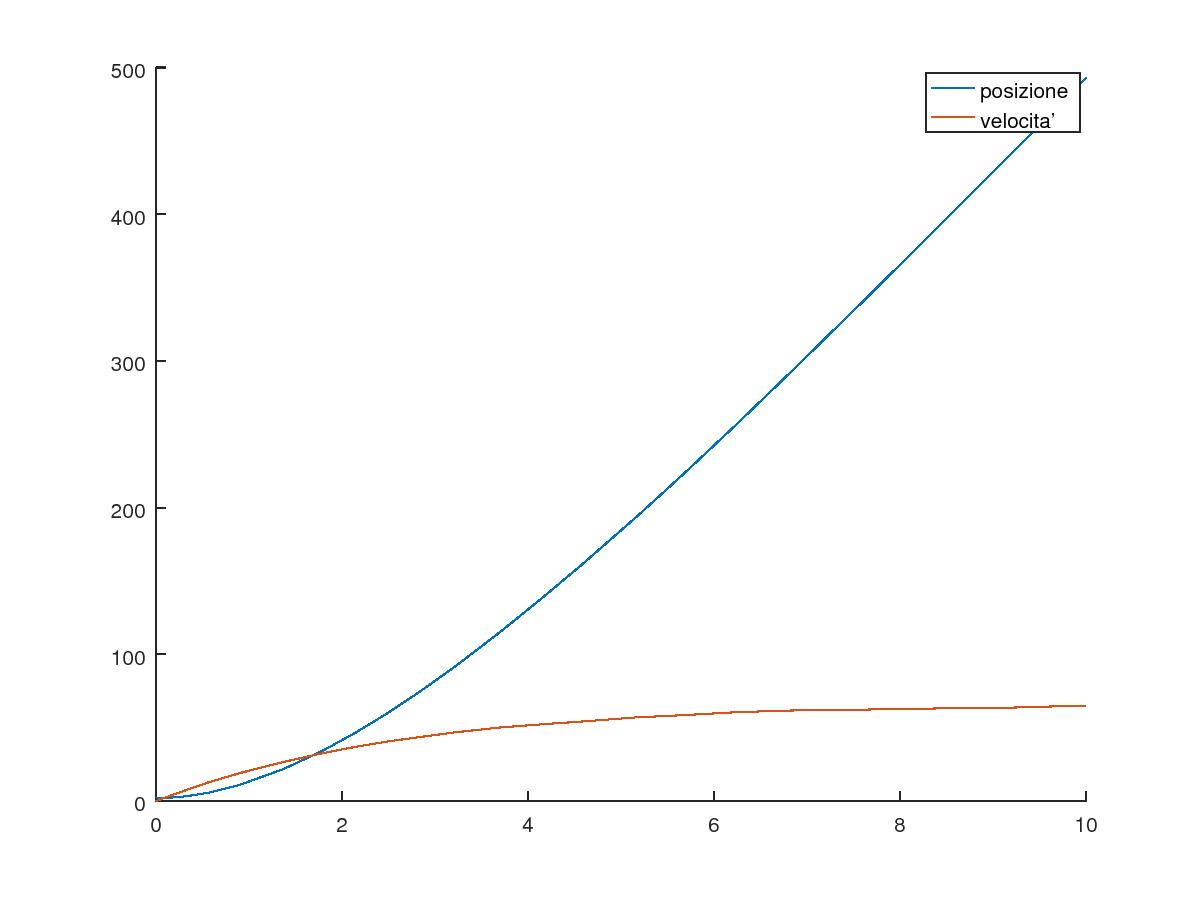
\includegraphics[width=0.7\textwidth]{5_4_4.jpeg}
	\end{figure}
\end{document}